\documentclass[a4paper,10pt]{article}
\usepackage{inputenc}
\usepackage{fancyhdr}
\usepackage{graphics}
\usepackage{amsmath}    % need for subequations
\usepackage{graphicx}   % need for figures
\usepackage{verbatim}   % useful for program listings
\usepackage{color}      % use if color is used in text
\usepackage{subfigure}  % use for side-by-side figures
\usepackage{hyperref}   % use for hypertext links, including those to external
\usepackage[spanish]{babel}

\pagestyle{fancy}

\lhead[\thepage]{Grupo N\'umero 2}      % Note the different brackets!
\rhead[Grupo N\'umero 2]{Julio 2010}

%opening
\title{Trabajo Pr\'actico Final\\Rally Uribe 100K\\}
\author{Guillermo Campelo\\Juan Ignacio Go\~ni\\Juan
Tenaillon\\Santiago Vazquez}

\begin{document}

\maketitle


\begin{abstract}
El siguiente informe describimos como dise\~namos e implementamos el
\textbf{Rally
Uribe
100K}. 
Mediante el uso de im\'agenes describimos c\'omo fueron dise\~nadas e
implementadas
las distintas partes que componen al total de la aplicaci\'on.  Tambi\'en
presentaremos los inconvenientes que surgieron a lo largo del desarrollo y
c\'omo decidimos solucionarlos.  Por \'ultimo explicaremos c\'omo se utiliza
el
juego,
c\'omo se modifican las distintas opciones de configuraci\'on del mismo y las
conclusiones.
\end{abstract}

\pagebreak
\tableofcontents
\pagebreak

\section{Introducci\'on}

Haciendo uso del Framework JMonkey, dise\~namos e implementamos un juego de
rally,
llamado Rally Uribe 100K.  A continuaci\'on, se describe c\'omo fue realizado el
mismo, qu\'e caracter\'isticas posee y la forma en que se utiliza.

Para el dise\~no e implementaci\'on del juego, partimos de la base del ejemplo
proporcionado por el Framework utilizado, y tomando esa base, realizamos
el desarrollo de las nuevas caracter\'isticas.

En la secci\'on \ref{el_juego} explicaremos c\'omo es el juego, los distintos
estados, c\'omo es el sistema de puntaje y los sonidos del mismo.

En la secci\'on \ref{caracteristicas} explicaremos qu\'e caracter\'i�sticas
adicionales desarrollamos para el juego, como las texturas procedurales,
los screenshots, los arbustos billboard, los skybox intercambiables y dem\'as.

En la secci\'on \ref{mododeuso} explicaremos c\'omo se utiliza el juego,
explicando
las teclas a utilizar por defecto, adem\'as explicaremos c\'omo utilizar las
distintas opciones del men\'u.

En la secci\'on \ref{configuracion} mostraremos las distintas opciones de
configuraci\'on, as\'i como los valores recomendados para la misma.  Tambi\'en
explicaremos c\'omo definir nuevas pistas, para que el usuario del mismo pueda
crear
sus propios recorridos y utilizarlos con el juego.

Por \'ultimo, en la secci\'on \ref{conclusiones} presentamos las
conclusiones que alcanzamos, adem\'as de posibles
extensiones al mismo y la
ense\~nanza obtenida del dise\~no y desarrollo del mismo.

\section{El Juego}
\label{el_juego}

En esta secci\'on explicaremos el juego como tal.  El objetivo, el
modo
de
juego, los distintos estados, c\'omo es el sistema de puntajes y los sonidos
del mismo.

\subsection{Descripci\'on}
El juego consiste en recorrer una pista de carreras, ambientada como si fuera
de Rally.  El ambiente en el cual se mueve el auto, est\'a compuesto de un
terreno, con una pista delimitada, con un conjunto de objetos que la componen.

El objetivo del mismo, es dar tres vueltas al recorrido propuesto.  Adem\'as de
completar la totalidad de las vueltas, el jugador debe transitar por la
totalidad de los checkpoints, en el orden determinado por la pista.  En caso de
saltearse uno el juego no le permitir\'a transitar exitosamente por los
siguientes, y el jugador deber\'a volver hacia atr\'as y transitar por el
checkpoint adeudado.

Al inicio, el auto se encuentra estacionado en su $box$.  Se decidi\'o esto
debido a que en el Rally, los autos no necesariamente realizan un recorrido
cerrado, y no arrancan desde una grilla de partida comun y corriente como en la
f\'ormula 1,  sino que arrancan solos y desde un lugar predeterminado por la
organizaci\'on. Es por eso que nosotros elegimos que el auto arranque en ese
lugar, tambi\'en llamado $boxes$.

Al finalizar las tres vueltas, el jugador recibir\'a el tiempo de su recorrido,
y
mientras m\'as bajo sea ese tiempo, m\'as chances tendr\'a de ingresar al
listado
de
los puntajes m\'as altos.
\subsection{Modo de Juego}
Hay un solo modo de juego, y este consiste en intentar realizar el menor tiempo
posible en la realizaci\'on de las tres vueltas a la pista.  Como comentamos
con antelaci\'on, es necesario transitar en el orden establecido a trav\'es de
los checkpoints para poder terminar con el recorrido.
\subsection{Estados del Juego}
Hay tres estados diferenciados en el juego.  Antes de comenzar a jugar, durante
el juego y luego de jugar.

Antes de comenzar a jugar, el jugador encuentra el men\'u principal de la
aplicaci\'on, el cual le presenta todas las opciones disponibles.  Una vez que
el
usuario selecciona la opci\'on para comenzar a jugar, realizamos la transici\'on
al
siguiente estado, el juego en s\'i.

\begin{figure}
\begin{minipage}[b]{0.5\linewidth}
\centering
 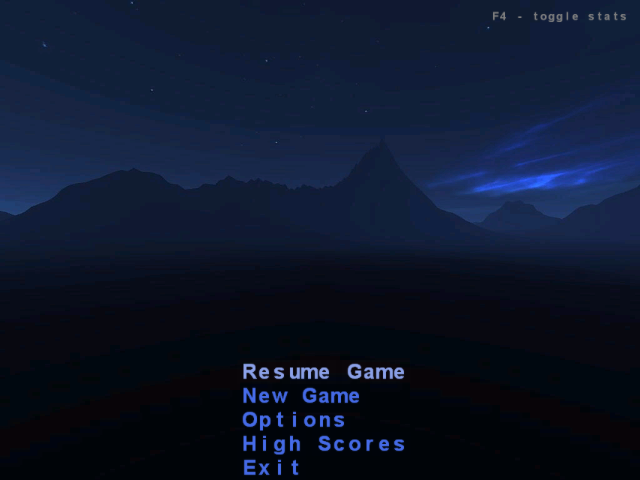
\includegraphics[scale=0.250]{./main_menu.png}
 % startinggrid.png: 640x480 pixel, 72dpi, 22.58x16.93 cm, bb=0 0 640 480
 \caption{Men\'u Principal.}
\label{fig:figure0}
\end{minipage}
\hspace{0.5cm}
\begin{minipage}[b]{0.5\linewidth}
\centering
 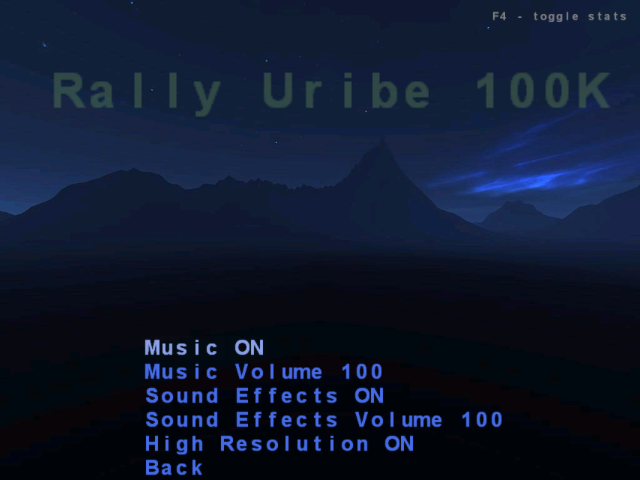
\includegraphics[scale=0.250]{./options_menu.png}
 % startinggrid.png: 640x480 pixel, 72dpi, 22.58x16.93 cm, bb=0 0 640 480
 \caption{Men\'u de Opciones.}
\label{fig:figure00}
\end{minipage}
\end{figure}

En este estado, es cuando el jugador maneja el veh\'iculo a trav\'es del camino
propuesto.  El veh\'iculo en esta ocasi\'on, puede colisionar contra los
distintos
objetos que componen la escena, como los \'arboles, los l\'imites del terreno y
las
pir\'amides presentes en el recorrido.  Una vez finalizado el recorrido,
realizamos la transici\'on al tercer y \'ultimo estado del juego.

En este tercer y \'ultimo estado, le presentamos al usuario el men\'u
nuevamente,
donde podr\'a ver los puntajes m\'aximos hasta el momento o comenzar nuevamente
el
juego para tratar de mejorar su tiempo.

\subsection{Puntajes}
El juego tiene la opci\'on de ver quienes fueron los jugadores que realizaron
los
diez mejores tiempo en el recorrido a la pista.

Una vez finalizado el recorrido, le presentamos al jugador su tiempo total
de
recorrido, y si el tiempo es lo suficientemente bueno el mismo ingresa en la
lista de los mejores tiempos, donde el identificador es la fecha en que fue
realizado el record.

En el men\'u inicial del juego, el jugador puede elegir la opci\'on de
$highscores$,
para ver cuales son los mejores tiempos a la pista y cuando lo realiz\'o.


\subsection{Sonidos}
El juego, como todos los de su tipo, tiene diferentes sonidos que ayudan a
ambientar el mismo.

Comenzando por los sonidos de ambiente, donde decidimos que se iban a
utilizar
dos pistas para tener cierto cambio en la m\'usica de ambiente pero sin entrar
en
la exageraci\'on de utilizar muchas.

Tambi\'en fueron utilizados dos sonidos para ser utilizados por el veh\'iculo
para
denotar situaciones en las que se est\'a acelerando y situaciones en las que no.

Por \'ultimo, utilizamos un sonido para los momentos en que el veh\'iculo
colisiona contra algun objeto presente en el terreno.

Todos los sonidos propios del veh\'iculo y su entorno fueron obtenidos de
Internet, de p\'aginas de uso libre y gratuito.  Los temas utilizados para la
m\'usica ambiental, corresponden a la autor\'ia de Santiago Vazquez, integrante
del
equipo.

\begin{figure}
\begin{minipage}[b]{0.5\linewidth}
\centering
 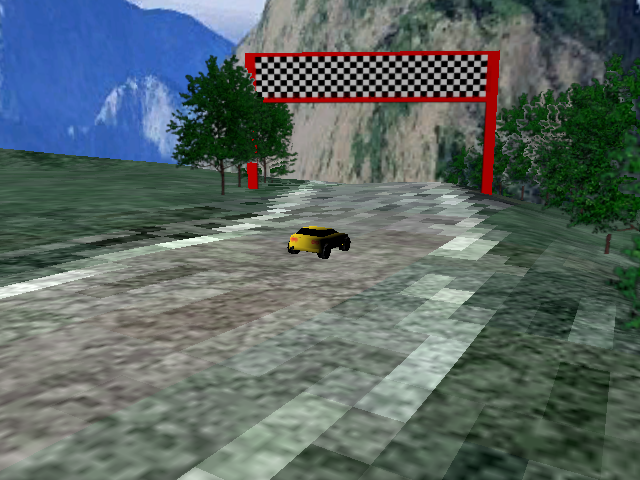
\includegraphics[scale=0.250]{./startinggrid.png}
 % startinggrid.png: 640x480 pixel, 72dpi, 22.58x16.93 cm, bb=0 0 640 480
 \caption{Grilla de Partida del Rally Uribe 100K. Bajo nivel de detalle.}
\label{fig:figure1}
\end{minipage}
\hspace{0.5cm}
\begin{minipage}[b]{0.5\linewidth}
\centering
 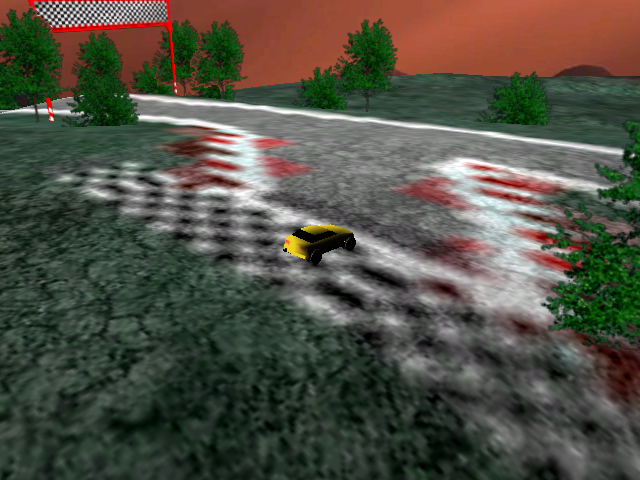
\includegraphics[scale=0.250]{./startinggrid_high.png}
 % startinggrid.png: 640x480 pixel, 72dpi, 22.58x16.93 cm, bb=0 0 640 480
 \caption{Grilla de Partida del Rally Uribe 100K. Alto nivel de detalle.}
\label{fig:figure2}
\end{minipage}
\end{figure}

\subsection{Iluminaci\'on}

El terreno en el cual se desarrolla el juego, cuenta con tres tipos distintos de
iluminaci\'on: una luz ambiente, una luz direccional y cinco luces puntuales que
iluminan la totalidad del recorrido.

La iluminaci\'on ambiente, est\'a configurada por defecto para tener un nivel
bajo de iluminaci\'on.  Elegimos esto para que el resto de las luces tomen un
papel m\'as importante en la iluminaci\'on del escenario.

Los valores de rojo, verde, azul y canal alfa que determinan la intensidad y
color de la luz, son f\'acilmente configurables en el archivo
$global.properties$, bajo el elemento $TRACK1.AMBIENT.LIGHT$.

La luz direccional la configuramos por defecto con un color rojo intenso y
est\'a emplazada encima del primer checkpoint del recorrido. La raz\'on de esta
decisi\'on radica en que ten\'iamos que buscar un lugar donde la luz fue
visible para demostrar la existencia de la misma, es por eso que cada vez que
el auto transita por debajo de la grilla de partida, se puede ver un color
rojizo en el techo del mismo.

Esta luz es tambi\'en configurable en cuanto a los colores rojo, verde, azul y
el canal alfa.  Para configurar esto, es necesario modificar en el archivo de
configuraci\'on, las propiedades que se encuentran bajo el elemento
$TRACK1.LIGHT.SPOTLIGHT$.

Por \'ultimo, las luces puntuales.  Las cinco luces puntuales est\'an en
distintos lugares a lo largo del recorrido.  A diferencia de los otros dos
tipos de iluminac\'on, estos tienen una posici\'on determinada por el usuario y
est\'an configuradas para dar una luz blanca.

Tanto la posici\'on de la luz como el color, son configurables.  Al igual que
el resto de las luces, para cambiar la posici\'on y color de estas, hay que
modificar las propiedades de cada luz en el archivo de configuraci\'on.  Cada
luz puntual est\'a contemplada bajo la propiedad $TRACK1.POINTLIGHTn$ donde $n$
es el n\'umero de la luz.

En las figuras \ref{fig:sinluz} y \ref{fig:conluz} apreciamos el juego
con las luces puntuales deshabilitadas y con las luces puntuales habilitadas
respectivamente.  Cabe destacar que en la figura \ref{fig:sinluz} observamos una
luz ambiental muy tenue junto con la luz direccional en color
rojo apuntando hacia abajo sobre el primer checkpoint.

\begin{figure}
\begin{minipage}[b]{0.5\linewidth}
\centering
 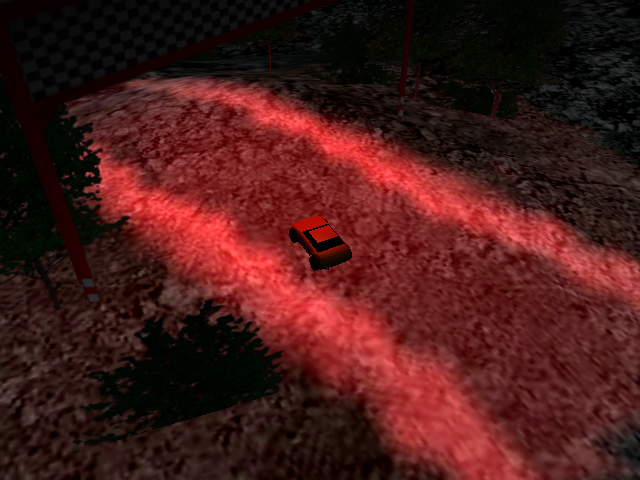
\includegraphics[scale=0.250]{./sinluz.png}
 % startinggrid.png: 640x480 pixel, 72dpi, 22.58x16.93 cm, bb=0 0 640 480
 \caption{Juego con luz ambiental tenue y luz direccional roja.}
\label{fig:sinluz}
\end{minipage}
\hspace{0.5cm}
\begin{minipage}[b]{0.5\linewidth}
\centering
 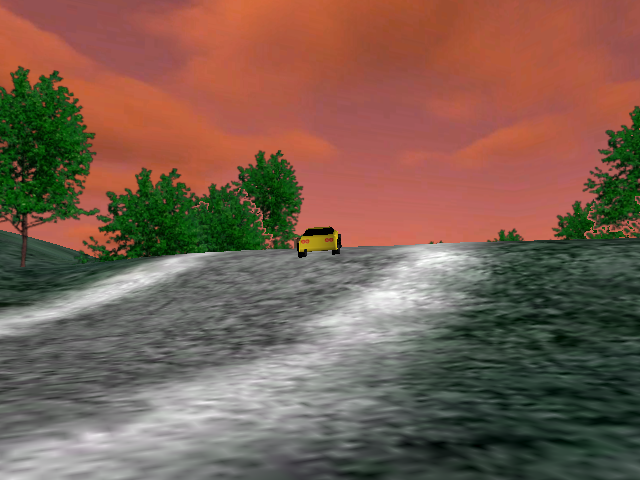
\includegraphics[scale=0.250]{./conluz.png}
 % startinggrid.png: 640x480 pixel, 72dpi, 22.58x16.93 cm, bb=0 0 640 480
 \caption{Juego con todas las luces habilitadas.}
\label{fig:conluz}
\end{minipage}
\end{figure}



\section{Caracter\'isticas Extra}
\label{caracteristicas}

Dentro de las caracter\'isticas opcionales a implementar, nos inclinamos
por las siguientes: texturas procedurales, capturas de pantallas, \'arboles con
billboards, diferentes skyboxes, c\'amaras est\'aticas, velocimetro y mapa de
posicionamiento.


\subsection{Texturas Procedurales}

Para la realizaci\'on de las texturas procedurales, el desarrollo fue basado en
el dise\~nado para la extensi\'on del \textit{Trabajo Pr\'actico N\'umero 2 -
Ray
Tracer}.  Se implementaron dos texturas procedurales, piedra y marmol.

\begin{figure}
\begin{minipage}[b]{0.5\linewidth}
\centering
 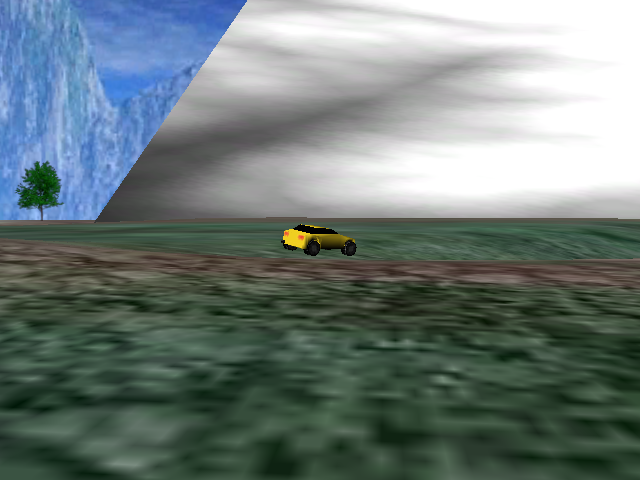
\includegraphics[scale=0.250]{./marble.png}
 % startinggrid.png: 640x480 pixel, 72dpi, 22.58x16.93 cm, bb=0 0 640 480
 \caption{Textura Procedural: Marmol.}
\label{fig:figure5}
\end{minipage}
\hspace{0.5cm}
\begin{minipage}[b]{0.5\linewidth}
\centering
 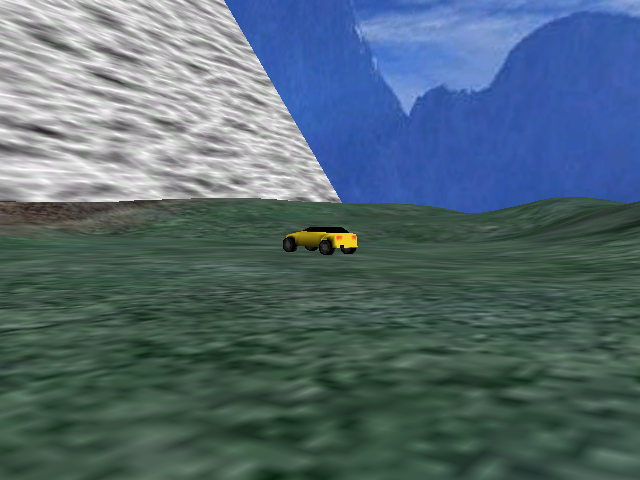
\includegraphics[scale=0.250]{./stone.png}
 % startinggrid.png: 640x480 pixel, 72dpi, 22.58x16.93 cm, bb=0 0 640 480
 \caption{Textura Procedural: Piedra}
\label{fig:figure6}
\end{minipage}
\end{figure}

Donde en la figura \ref{fig:figure5} y \ref{fig:figure6} se puede observar las
dos texturas procedurales realizadas, marmol y piedra respectivamente.

Para las mismas, utilizamos Perlin Noise.  Para m\'as detalle,
remitirse al informe del \textit{Trabajo Pr\'actico N\'umero 2 - Extensi\'on}.

\subsection{Capturas de Pantalla}

Otra de las caracter\'isticas que desarrollamos, fue la posibilidad de obtener
capturas de pantallas en cualquier momento del juego.  Para realizar dicha
acci\'on, hay que presionar la tecla $0$ (cero) en cualquier momento del
mismo.
Las im\'agenes producidas, son almacenadas en la carpeta $screenshots$
presente en la ra\'iz del proyecto, y el
nombre
con el que se guardan es la fecha en que fueron realizadas.

Esta caracter\'istica la utilizamos mucho a la hora de realizar este informe.

\subsection{Billboards}

Otra caracter\'istica que implementamos, fue el hecho de contar con \'arboles y
arbustos realizados con $billboards$ que nos provey\'o el Framework de JME.

En las im\'agenes presentadas con antelaci\'on y m\'as precisamente en la figura
\ref{fig:figure7}, puede observarse c\'omo este tipo de \'arboles son utilizados
a lo largo de todo el recorrido; donde tambi\'en cabe mencionar que el
veh\'iculo
puede colisionar contra este tipo de texturas.

Algo interesante sobre este tipo de texturas es que nos brindan la posibilidad
de verlas correctamente desde cualquier \'angulo, adem\'as permitiendo que se
vean con claridad las otras texturas detras de ellas.

\begin{figure}
 \centering
 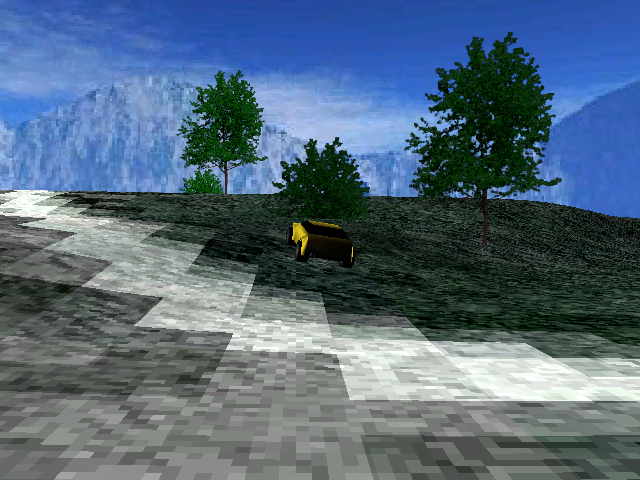
\includegraphics[scale=0.4]{./billboard.png}
 % billboard.png: 640x480 pixel, 72dpi, 22.58x16.93 cm, bb=0 0 640 480
 \caption{\'Arboles y arbustos billboard.}
 \label{fig:figure7}
\end{figure}

La diferencia entre los \'arboles y los arbustos, es que estos \'ultimos no son
colisionables.  Es decir, uno puede atravesar un arbusto pero uno no
puede atravesar un \'arbol ya que se chocar\'ia con el tronco del mismo.

En el escenario presentado por defecto, hay \'arboles y arbustos alternados.

\subsection{Uso y Selecci\'on de distintos \textit{Skyboxes}}

Uno de los opcionales seleccionados para el desarrollo del juego, fue darle al
usuario la posibilidad de elegir distintos skyboxes.  Se ofrecen tres, uno para
el d\'ia, otro para la tarde y el \'ultimo para la noche.

Cuando el jugador selecciona la opci\'on de $New Game$, tiene la posibilidad de
seleccionar el momento del d\'ia en que quiere correr la carrera.  Esto se
ver\'a reflejado en la carrera en si, una vez que comience la misma.  En todas
las im\'agenes presentes en el informe, se puede apreciar el skybox que
pertenece al momento \textit{d\'ia} mientras que en la figura \ref{fig:conluz}
se puede apreciar un cielo rojizo, simulando el atardecer.

\subsection{C\'amaras Est\'aticas}

A lo largo de la carrera, el jugador puede presionar la tecla $C$ y esto va a
cambiar la c\'amara desde donde se ve la carrera.  En cada checkpoint hay una
c\'amara est\'atica que est\'a apuntando al mismo.

En la figura \ref{fig:static} observamos una c\'amara est\'atica en el
segundo checkpoint.

\begin{figure}
 \centering
 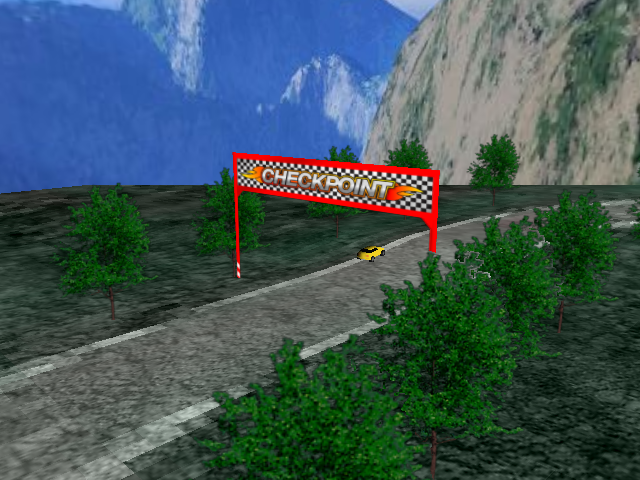
\includegraphics[bb=0 0 640 480,scale=0.4,keepaspectratio=true]{./static.png}
 % static.png: 640x480 pixel, 72dpi, 22.58x16.93 cm, bb=0 0 640 480
 \caption{C\'amara est\'atica en el segundo checkpoint}
 \label{fig:static}
\end{figure}

\subsection{Mapa de Posicionamiento}

Otra caracter\'istica que decidimos implementar, fue el mapa de posicionamiento
en pantalla.  Durante el juego, est\'a presente un mapa en la parte inferior
izquierda que nos indica la posici\'on en la que estamos.

En este mapa se pueden diferenciar tres tipos de puntos bien diferenciados. 
Con amarillo, el auto del jugador, con color rojo, la grilla de partida y con
color naranja, los distintos checkpoints presentes a trav\'es de la pista.

En la figura \ref{fig:game} observamos, abajo a la izquierda, el mapa de
posicionamiento en la pista.

\subsection{Calidad de los gr\'aficos}

Otra caracter\'istica que implementamos como opcional fue la posibilidad de
determinar la calidad de las im\'agenes que se presentaban en el juego
como podemos apreciar en las figuras \ref{fig:figure1} y \ref{fig:figure2}.
En el menu de opciones podemos elegir si queremos jugar en alta o baja
calidad.

Con este par\'ametro determinamos la cantidad de \'arboles y arbustos que
agregamos a la pista, la cantidad de obst\'aculos, el campo visual de la
c\'amara y uno de los factores m\'as importantes, la calidad de las texturas.

Esta \'ultima caracter\'istica fue vital para poder ejecutar el juego en
computadoras cuyas placas de video no eran de gama media o alta.

\subsection{Veloc\'imetro}

El \'ultimo opcional que decidimos implementar, fue el velocimetro con una
aguja.  Para realizar esto, utilizamos una imagen de un velocimetro sin la
aguja, y un cuadrilatero por separado.  Una vez que tuvimos esto, lo
posicionamos en su lugar y luego le aplicamos a la aguja, una rotaci\'on
dependiendo de la velocidad actual de veh\'iculo.

Dependiendo de la velocidad lineal del veh\'iculo, hacemos una traducci\'on de
ese valor lineal a un \'angulo entre $-112.5$ y $112.5$ grados, que nos da la
rotaci\'on de la aguja para un velocimetro que tolera velocidades entre 0 y 160
millas por hora.

En la figura \ref{fig:game} observamos, abajo a la derecha, el
veloc\'imetro del auto.


\begin{figure}
 \centering
 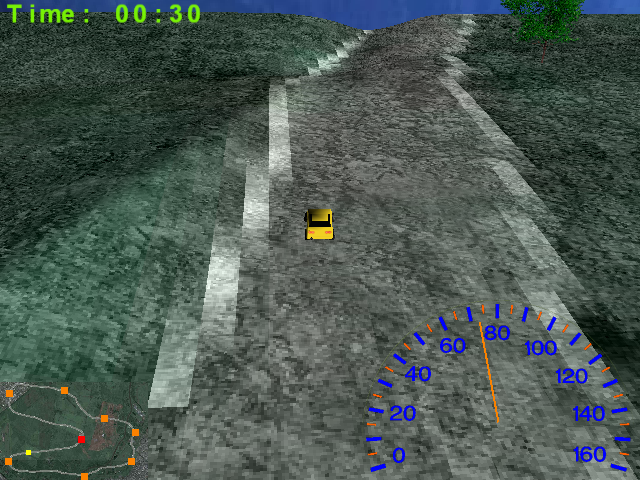
\includegraphics[bb=0 0 640 480,scale=0.4,keepaspectratio=true]{./game.png}
 % game.png: 640x480 pixel, 72dpi, 22.58x16.93 cm, bb=0 0 640 480
 \caption{El Juego.}
 \label{fig:game}
\end{figure}


\section{Modo de Uso}
\label{mododeuso}
En esta secci\'on, comentaremos la forma de jugar al Rally Uribe 100K.  Cabe
destacar que estas instrucciones est\'an basadas en la configuraci\'on default
del
juego, ya que cabe la posibilidad de modificar las teclas a utilizar.

\subsection{¿C\'omo se Juega?}
Para jugar al juego, solo es necesario conocer las teclas para moverse a traves
de la pista.  Lo \'unico necesario es saber con qu\'e teclas avanzar,
retroceder,
girar a la izquierda y a la derecha.  Luego, solo es necesario atravesar los
diferentes checkpoints hasta llegar a la meta.

Por defecto, las teclas para mover el vehiculo a traves del terreno son las
flechas hacia arriba para acelerar, hacia abajo para desacelerar y ir hacia
atras, hacia la izquiera para doblar en esa direcci\'on y hacia la derecha para
doblar a la derecha.

Durante el juego, es posible pausar el mismo mediante la tecla $P$, ir al
men\'u preseionando la tecla $ESC$ y sacar
$screenshots$ con la tecla $0$.

Adem\'as, es posible cambiar la c\'amara con la que se ve el veh\'iculo a otras
c\'amaras est\'aticas mediante la tecla $C$.

En el caso que el auto vuelque podemos volver al \'ultimo checkpoint mediante
la tecla $S$. En el caso que no hayamos pasado por ninguno, nos llevar\'a a la
l\'inea de partida.

\subsection{Los Men\'ues}
Para movernos a trav\'es de los men\'ues, es necesario utilizar las flechas
hacia
arriba, abajo, izquierda, derecha y el enter.  Con las flechas de arriba y
abajo, marcaremos la opci\'on deseada, mientras que con la tecla de enter,
seleccionaremos la misma.

En las opciones del men\'u que contengan distintas posibilidades de
configuraci\'on, ya sea el momento del d\'ia en cual vamos a correr, estado del
sonido y dem\'as opciones, es necesario utilizar las flechas hacia la derecha e
izquierda para cambiar la opci\'on.
\section{Configuraci\'on}
\label{configuracion}
El juego, como mencionamos con antelaci\'on, tiene ciertas caracter\'isticas
que
son configurables.  Desde las teclas, las texturas de los skyboxes, las
caracter\'isticas de las pistas y las pistas en s\'i son configurables.

Todas estas caracter\'isticas configurables, pueden ser modificadas desde el
archivo $global.properties$.

\subsection{Configuraci\'on del Juego}

Desde el archivo previamente mencionado, es posible configurar todas las teclas
del juego adem\'as de los nombres y texturas de los skyboxes, el estado de la
m\'usica y los efectos como las pistas a escucharse ante cada evento y/o pistas
de la m\'usica ambiental.  Adem\'as, tanto para la m\'usica como para los
efectos,
es
posible configurar en qu\'e nivel quiere uno que se encuentren, del 0 al 100,
siendo 100 el volumen m\'as alto de la m\'usica o efecto.

\subsection{Teclas}

Desde el archivo de configuraci\'on es posible modificar las teclas que van a
ser utilizadas para jugar al juego.  Las teclas vienen configuradas por
defecto, pero modificando los valores en el archivo $global.properties$ es
posible modificarlas.

\begin{verbatim}
SCREENSHOT=0B
PAUSE=19
CAMERA=2E
EXIT=01
RETURN=1F
FORWARD=C8
BACKWARD=D0
STEERLEFT=CB
STEERRIGHT=CD
ARROWUP=C8
ARROWDOWN=D0
ARROWLEFT=CB
ARROWRIGHT=CD
SELECT=1C
\end{verbatim}

Los valores que tiene cada opci\'on, son un n\'umero hexadecimal que est\'a
mapeado a una tecla.  Se eligi\'o esta configuraci\'on por que es la que maneja
la clase de Java que nos brinda esta funcionalidad.

Tanto las teclas para mover el veh\'iculo en el juego como las teclas para
moverse en el men\'u, est\'an configuradas de la misma forma.  Esto es debido a
que utilizan las flechas del teclado.  Tambi\'en ser\'ia posible si el usuario
quisiera, cambiar las teclas con las que maneja el veh\'iculo o las teclas con
las que se mueve en el men\'u.


\subsection{Configuraci\'on de Nuevas Pistas}

Desde el archivo de configuraci\'on, es posible determinar la posici\'on de los
distintos objetos que componen a la escena.

Los \'arboles, checkpoints, pir\'amides con texturas procedurales, como el resto
de
los objetos presentes, pueden ser configurados f\'acilmente desde el archivo de
configuraci\'on.

Para configurar los \'arboles presentes en la escena, es necesario indicar qu\'e
cantidad de \'arboles habr\'a, y acto seguido, indicar para cada uno de esos
\'arboles, que posici\'on van a ocupar en el terreno.

Un ejemplo del archivo de configuraci\'on para la determinaci\'on de la
posici\'on
de
los \'arboles es:

\begin{verbatim}
TRACK1.TREE.COUNT=425
TRACK1.TREE1.POS=672, -846
TRACK1.TREE2.POS=664, -859
TRACK1.TREE3.POS=642, -889
...
TRACK1.TREE425.POS=1642, -1889
\end{verbatim}

Donde se puede observar c\'omo en la primera l\'inea, se le indica la cantidad
de
\'arboles presentes en la escena y luego, para cada uno de los \'arboles, una
posici\'on dada por dos puntos.

Para el caso de los checkpoints, es similar a los \'arboles pero con una
peque\~na
variaci\'on, dada por la necesidad de determinar la rotaci\'on del plano que
contiene al checkpoint.

Un ejemplo del archivo de configuraci\'on para la determinaci\'on de la
posici\'on
de
los checkpoints es:

\begin{verbatim}
TRACK1.CHECKPOINT.COUNT=8
TRACK1.CHECKPOINT1.POS=515,-806
TRACK1.CHECKPOINT1.ROT=6.68925
TRACK1.CHECKPOINT2.POS=-4434,-3150
TRACK1.CHECKPOINT2.ROT=6.32625
TRACK1.CHECKPOINT3.POS=694,-4591
TRACK1.CHECKPOINT3.ROT=4.748
TRACK1.CHECKPOINT4.POS=3880,-3081
TRACK1.CHECKPOINT4.ROT=3.604
TRACK1.CHECKPOINT5.POS=4094,-138
TRACK1.CHECKPOINT5.ROT=3.126
TRACK1.CHECKPOINT6.POS=2069,1334
TRACK1.CHECKPOINT6.ROT=7.718
TRACK1.CHECKPOINT7.POS=-674,4184
TRACK1.CHECKPOINT7.ROT=2.126
TRACK1.CHECKPOINT8.POS=-4363,3862
TRACK1.CHECKPOINT8.ROT=6.451
\end{verbatim}

Donde aca podemos observar como est\'an presentes los 8 checkpoints utilizados
en
la pista presentada, donde cada uno tiene su posici\'on y su rotaci\'on en
radiantes.

Otra posibilidad ser\'ia la de configurar las pir\'amides con texturas
procedurales.  De forma similar que los ejemplos presentados con antelaci\'on,
un
ejemplo de una entrada en el archivo de configuraci\'on ser\'ia:

\begin{verbatim}
TRACK1.PIRAMID.COUNT=2
TRACK1.PIRAMID1.POS=2858,2142
TRACK1.PIRAMID1.TYPE=Marble
TRACK1.PIRAMID2.POS=1850,-150
TRACK1.PIRAMID2.TYPE=Stone
\end{verbatim}

Donde adem\'as de indicar la cantidad de pir\'amides que van a haber en el
terreno,
es necesario indicarle que textura utilizaran.  Previamente en el informe
comentamos la existencia de dos tipos de texturas procedurales, piedra y
marmol, tal como se pueden apreciar en el archivo de configuraci\'on de la
pista.

Para realizar la pista, el Framework de JME nos provee de una funci\'on para
realizar terrenos.  Uno le indica la altura m\'axima y m\'inima y el terreno es
generado por el Framework.  Para modificar la textura del terreno, utilizamos
una imagen obtenida de Google Maps y modificada para que sea una pista de
carreras.  Hay dos archivos utilizados para la pista, $autodromo2.png$ y
$autodromo2low.png$.  El primero es la pista con alta nivel de detalle y el
segundo es la pista con un nivel de detalle m\'as bajo.

\section{Conclusi\'on}
\label{conclusiones}

A lo largo del desarrollo del juego, pudimos adquirir varios conceptos y
ense\~nanzas del proceso que conlleva crear y desarrollar uno.

Para comenzar, adquirimos conocimientos sobre las distintas partes que componen
a un juego, las distintas fases de los mismos y adem\'as, logramos adquirir
cierta experiencia utilizando un framework para el desarrollo de videojuegos en
Java.

Cabe destacar que debido a que decidimos utilizar JME2 para el
desarrollo
del juego, y que ante cada problema o situaci\'on en la que
requerimos asistencia,
logramos
sortear el inconveniente gracias a la extensa documentaci\'on sobre el Framework
que est\'a disponible en los distintos foros y en la misma documentaci\'on
propia
de los desarrolladores del mismo.

Por \'ultimo, tambi\'en nos parece valioso remarcar que a lo largo del
desarrollo nos encontramos con varias disyuntivas las que nos llevaron a
trabajar, discutir y decidir en equipo cual era la mejor soluci\'on para un
problema dado.  De esta forma, pudimos desarrollar nuestra capacidad
colaborativa y de trabajo en equipo.


\end{document}
